%!TEX root = ../main.tex

%!TEX root = ../main.tex

\RequirePackage{bibentry}
\makeatletter\let\saved@bibitem\@bibitem\makeatother

\documentclass{beamer}
\makeatletter\let\@bibitem\saved@bibitem\makeatother

\renewcommand{\baselinestretch}{1.2}\normalsize
\usetheme{default}
\setbeamertemplate{navigation symbols}{}
\setbeamertemplate{footline}[frame number]

\usepackage{verbatim}
\usepackage{etex}

% BIBLIOGRAPHY APACITE
\usepackage[apaciteclassic]{apacite}
\usepackage{notoccite}
\usepackage{bibentry}
\usepackage{pdfpages}

% MATHEMATICS AND FONTS
\DeclareMathOperator*{\argmin}{arg\,min}
\DeclareMathOperator*{\argmax}{arg\,max}

\renewcommand{\vec}[1]{\mathbf{#1}}

\usepackage{amsfonts}
\usepackage{amsmath}
\usepackage{amssymb}
\usepackage{bbm}
\usepackage{algpseudocode}
\usepackage{setspace}

\usepackage{arev}
\usepackage[latin1]{inputenc}
\usepackage[T1]{fontenc}

\definecolor{darkblue}{rgb}{0,.35,.62}
\definecolor{lightblue}{rgb}{0.8,0.85,1}
\definecolor{lightgrey}{gray}{0.1}	%Farben mischen
\definecolor{Gray}{gray}{0.9}
\definecolor{mplorange}{HTML}{FF7F0E}
\definecolor{mplred}{HTML}{D62728}
\definecolor{mplblue}{HTML}{1F77B4}
\definecolor{mplgreen}{HTML}{2CA02C}

% GRAPHS
\usepackage{graphicx}
\usepackage{subfig}
\usepackage{caption}
\graphicspath{{material/}}
\usepackage{relsize}
\usepackage{lscape}
\usepackage{fancybox}
\usepackage{epstopdf}


% TABLES AND OTHER ENVIRONMENTS
\usepackage{tabularx}
\usepackage{longtable}
\usepackage{booktabs}
\usepackage{color,colortbl}
\usepackage{threeparttable}

\usepackage{enumerate}

\usepackage{fix-cm}

\usepackage{bookmark}
\usepackage{hyperref}
\hypersetup{colorlinks=true,urlcolor=blue,citecolor=black}


\usepackage{tikz}
\tikzset{
	treenode/.style = {shape=rectangle, rounded corners,
		draw, align=center,
		top color=white, bottom color=blue!20},
	root/.style     = {treenode, font=\Large, bottom color=red!30},
	env/.style      = {treenode, font=\ttfamily\normalsize},
	dummy/.style    = {circle,draw}
}
%\usepackage{cmbright}
\def\newblock{\hskip .11em plus .33em minus .07em}
\newcommand{\bs}{\boldsymbol}
\newcommand{\N}{\mathbb{N}}
\newcommand{\cov}{\mathrm{cov}\thin}
\newcommand{\thin}{\thinspace}
\newcommand{\thick}{\thickspace}
\newcommand{\Lim}[1]{\raisebox{0.5ex}{\scalebox{0.8}{$\displaystyle \lim_{#1}\;$}}}

\newcommand{\vect}[1]{\mathbf{#1}}
\newcommand{\myfrac}[3][0pt]{\genfrac{}{}{}{}{\raisebox{#1}{$#2$}}{\raisebox{-#1}{$#3$}}}
\newcommand{\U}{\mathrm{U}}	%Uniform Distribution
\newcommand{\D}{\mathrm{D}}	%Dirichlet Distribution
\newcommand{\W}{\mathrm{W}}	%Wishart Distribution
\newcommand{\E}{\mathrm{E}}		%Expectation
\newcommand{\Prob}{\mbox{Pr}}		%Expectation
\newcommand{\Iden}{\mathbb{I}}	%Identity Matrix
\newcommand{\Ind}{\mathrm{I}}	%Indicator Function
\newcommand{\Tau}{\mathcal{T}\thin}

\newcommand{\var}{\mathrm{var}\thin}
\newcommand{\plim}{\mathrm{plim}\thin}
\newcommand\indep{\protect\mathpalette{\protect\independenT}{\perp}}
\def\independenT#1#2{\mathrel{\rlap{$#1#2$}\mkern5mu{#1#2}}}
\newcommand{\notindep}{\ensuremath{\perp\!\!\!\!\!\!\diagup\!\!\!\!\!\!\perp}}%

\newcommand{\mc}{\multicolumn}

\newcommand{\ph}{\phantom}
% weitere Optionen:
% secbar: Gliederung im Kopf, nur sections (alternativ zu subsecbar)
% handout: Produktion von Handouts, keine Animationen
\definecolor{darkblue}{rgb}{0,.35,.62}
\definecolor{lightblue}{rgb}{0.8,0.85,1}
\definecolor{lightgrey}{gray}{0.1}	%Farben mischen

%	kbordermatrix options

\makeatletter
\newcommand{\vast}{\bBigg@{4}}
\newcommand{\Vast}{\bBigg@{5}}
\makeatother
\newcommand{\indicator}[1]{\mathbbm{1}{\left\{ {#1} \right\} }}
\newcommand{\indic}{1{\hskip -2.5 pt}\hbox{1} }


\definecolor{lightgrey}{gray}{0.90}	%Farben mischen
\definecolor{grey}{gray}{0.85}
\definecolor{darkgrey}{gray}{0.65}
\definecolor{lightblue}{rgb}{0.8,0.85,1}

\renewcommand{\arraystretch}{1.5}


\usepackage{tikz}
\usetikzlibrary{trees,shapes,arrows,decorations.pathmorphing,backgrounds,positioning,fit,petri}
\renewcommand*{\familydefault}{\sfdefault}

\tikzset{forestyle/.style = {rectangle, thick, minimum width = 5cm, minimum height = 0.5cm, text width = 4.5cm, outer sep = 1mm},
	pre/.style={<-, shorten <=1pt, >=stealth, ultra thick},
	extend/.style={<-,dashed, shorten <=1pt, >=stealth, ultra thick}}
\captionsetup[subfigure]{labelformat=empty}


\newcommand{\beginbackup}{
	\newcounter{framenumbervorappendix}
	\setcounter{framenumbervorappendix}{\value{framenumber}}
}
\newcommand{\backupend}{
	\addtocounter{framenumbervorappendix}{-\value{framenumber}}
	\addtocounter{framenumber}{\value{framenumbervorappendix}}
}


% Begin Full Justification ---------------------------------------------------------

\usepackage{ragged2e}
% \usepackage{etoolbox}
\usepackage{lipsum}
\makeatletter
\renewcommand{\itemize}[1][]{%
	\beamer@ifempty{#1}{}{\def\beamer@defaultospec{#1}}%
	\ifnum \@itemdepth >2\relax\@toodeep\else
	\advance\@itemdepth\@ne
	\beamer@computepref\@itemdepth% sets \beameritemnestingprefix
	\usebeamerfont{itemize/enumerate \beameritemnestingprefix body}%
	\usebeamercolor[fg]{itemize/enumerate \beameritemnestingprefix body}%
	\usebeamertemplate{itemize/enumerate \beameritemnestingprefix body begin}%
	\list
	{\usebeamertemplate{itemize \beameritemnestingprefix item}}
	{\def\makelabel##1{%
			{%
				\hss\llap{{%
						\usebeamerfont*{itemize \beameritemnestingprefix item}%
						\usebeamercolor[fg]{itemize \beameritemnestingprefix item}##1}}%
			}%
		}%
	}
	\fi%
	\beamer@cramped%
	\justifying% NEW
	%\raggedright% ORIGINAL
	\beamer@firstlineitemizeunskip%
}

\justifying

% \apptocmd{\frame}{\justifying}{}{}

\usepackage{array}
\newcolumntype{L}[1]{>{\raggedright\let\newline\\\arraybackslash\hspace{0pt}}m{#1}}
\newcolumntype{C}[1]{>{\centering\let\newline\\\arraybackslash\hspace{0pt}}m{#1}}
\newcolumntype{R}[1]{>{\raggedleft\let\newline\\\arraybackslash\hspace{0pt}}m{#1}}



% End Full Justification ------------------------------------------------------------


\title{Data Analytics with Python}
\author{Tobias Raabe}
\date{}
\let\otp\titlepage

\begin{document}
\maketitle

\begin{frame}[c]\frametitle{Table of Contents}
\tableofcontents
\end{frame}

\section{Why Python?} % (fold)
\label{sec:why_python}

\begin{frame}[c]\frametitle{Why Python?}
\begin{itemize}
    \item \textbf{open source} (you are able to review the source code)
    \item \textbf{easy to learn} (you are able to write your own code)
    \item \textbf{general-purpose language} (you are able to perform all actions ranging from creating folders to analyzing data)
    \item \textbf{glue language} (your are able to implement a variety of other programming language into a project like R, C, Julia, etc.)
    \item \textbf{increasing popularity among the economics and econometrics community}
    \item \textbf{fast growing}
\end{itemize}
\end{frame}

\begin{frame}[c]
\begin{figure}[tb]
    \centering
    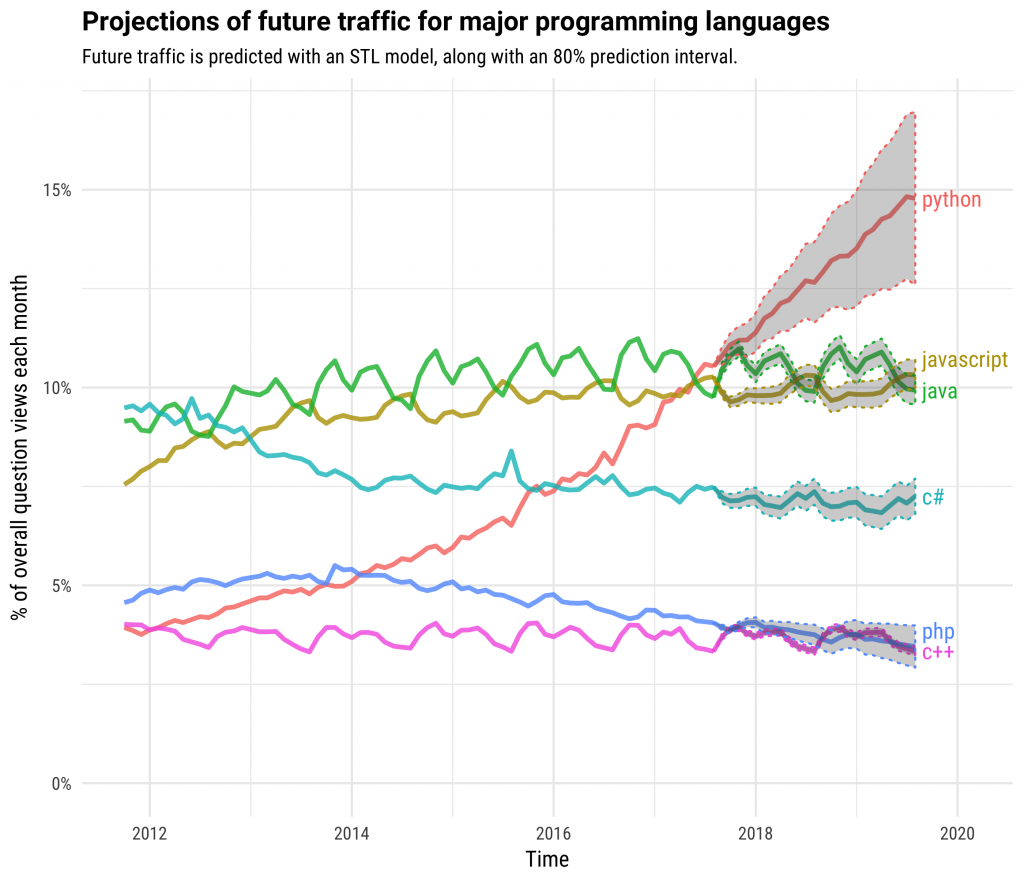
\includegraphics[width=0.8\textwidth, height=0.8\textheight]{../material/fig-python-growth}
    \caption{source: \url{https://stackoverflow.blog/2017/09/06/incredible-growth-python/}}
    \label{fig:python-growth}
\end{figure}
\end{frame}

\begin{frame}[c]
\begin{figure}[tb]
    \centering
    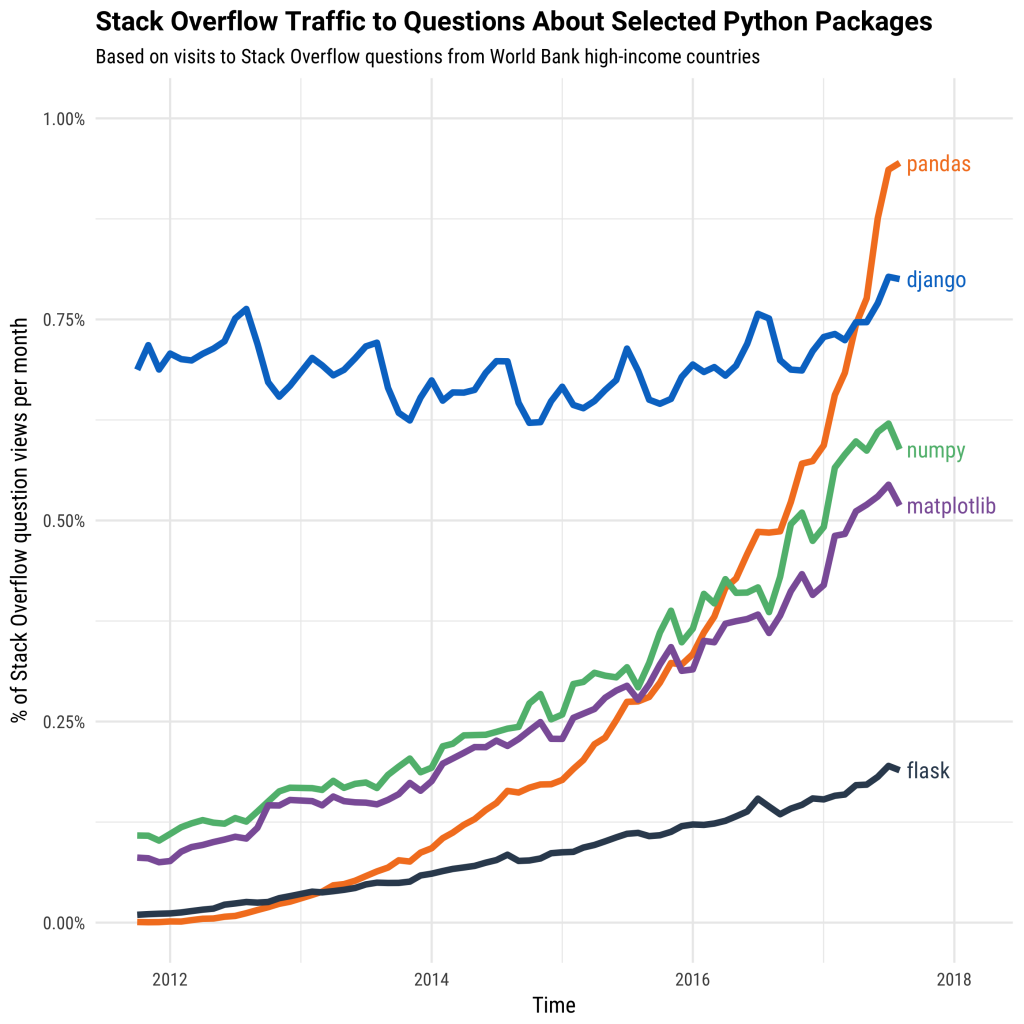
\includegraphics[width=0.8\textwidth, height=0.8\textheight]{../material/fig-pandas-growth}
    \caption{source: \url{https://stackoverflow.blog/2017/09/14/python-growing-quickly/}}
    \label{fig:pandas-growth}
\end{figure}
\end{frame}

\begin{frame}[c]
\begin{figure}[tb]
    \centering
    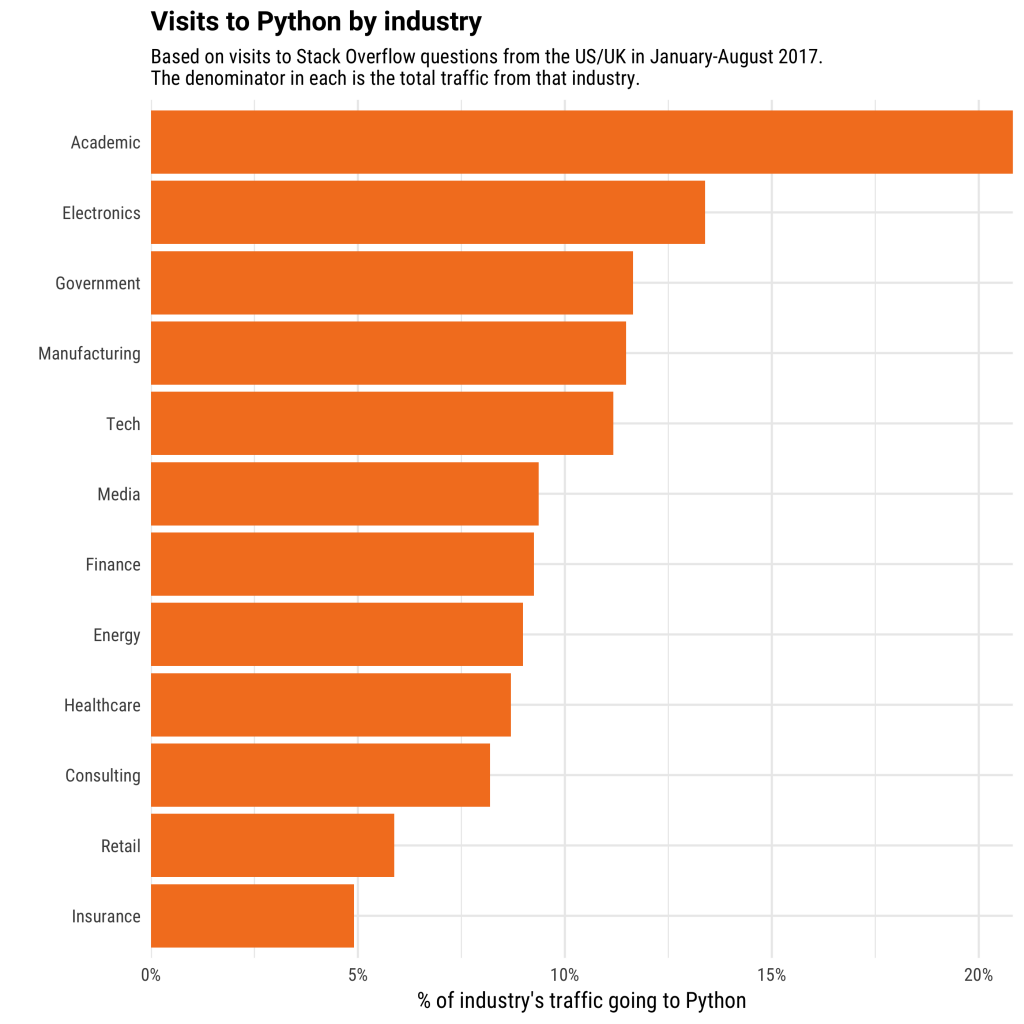
\includegraphics[width=0.8\textwidth, height=0.8\textheight]{../material/fig-pandas-visitors-by-industry}
    \caption{source: \url{https://stackoverflow.blog/2017/09/14/python-growing-quickly/}}
    \label{fig:figure1}
\end{figure}
\end{frame}
% section why_python (end)

\section{Why not R, or Stata} % (fold)
\label{sec:why_not_r_stata}

\begin{frame}[c]\frametitle{Why not R, Stata}
\begin{description}
    \item[R]
    \begin{itemize}
        \item major inspiration for most scientific Python packages
        \item \href{https://www.tidyverse.org/}{Tidyverse} is a collection of incredible powerful data analysis tools
        \item (my opinion: quirky syntax)
    \end{itemize}
    \item[Stata]
    \begin{itemize}
        \item proprietary and closed code base
        \item useful for quick analysis
        \item (my opinion: quirky syntax, hard to manage bigger projects, how to ensure reproducibility)
    \end{itemize}
\end{description}
\end{frame}
% section why_not_r_stata_matlab_julia (end)

\section{Scientific Computing Tools for Python} % (fold)
\label{sec:scientific_computing_tools_for_python}

\begin{frame}[c]\frametitle{Scientific Computing Tools for Python}
Packages\footnote{\url{https://www.scipy.org/about.html}}

\begin{description}
    \item[NumPy] fundamental package for numerical operations
    \item[SciPy] collection of numerical algorithms, statistics, optimizations, etc.
    \item[Matplotlib] plotting library
    \item[pandas] provides high-performance and easy-to-use data structures
    \item[scikit-learn] collection of algorithms and tools for machine learning
    \item[Jupyter] powerful IDE (integrated development environment) which combines python and markdown
    \item[Anaconda] an installer for a preconfigured python environment containing the scientific stack and many other useful libraries
\end{description}
\end{frame}
% section scientific_computing_tools_for_python (end)


\section{Setup} % (fold)
\label{sec:setup}

\begin{frame}[c]\frametitle{Setup}
\begin{enumerate}
    \item download the files required for the tutorial from \href{https://www.dropbox.com/sh/0onu61t2olg2gwz/AAAtqiANuKODdBDdPlGTYtXja?dl=0}{here}, unzip and place them into a folder in your user directory.
    \item download the installer for Python 3.6 from \url{https://www.anaconda.com/download/} and run it
    \begin{itemize}
        \item \textit{If you are asked whether Anaconda and its paths should be added to your system's PATH or not, choose the option to add them}
    \end{itemize}
    \item start the Jupyter notebook in one of two ways
    \begin{enumerate}
        \item use terminal, shell, cmd, powershell to navigate to your project's folder and enter \texttt{jupyter notebook}
        \item start Jupyter via the Anaconda Navigator (installed with Anaconda)
    \end{enumerate}
    \item make sure that you can navigate to the tutorial folder inside the opened tab in your browser
    \item (optional) Start a new notebook by clicking on \texttt{New} in the top right corner and select Python 3
\end{enumerate}
\end{frame}
% section setup (end)

\section{Useful links} % (fold)
\label{sec:useful_links}

\begin{frame}[c]\frametitle{Tutorials}
\begin{itemize}
    \item \href{https://learnpythonthehardway.org/}{Zed A. Shaw - Learn Python the Hard Way - General Python Tutorial}
    \item \href{https://blog.patricktriest.com/police-data-python/}{Patrick Triest - Exploring US Policing Data using Python}
\end{itemize}
\end{frame}

\begin{frame}[c]\frametitle{Documentation}
\begin{itemize}
    \item \href{https://stackoverflow.com/}{stackoverflow - World's largest developer community}
\end{itemize}
\end{frame}

\begin{frame}[c]\frametitle{Others}
\begin{itemize}
    \item \href{https://www.anaconda.com/download/}{Anaconda Distribution} delivers Python with a pre-compiled stack of scientific packages
    \item \href{https://jakevdp.github.io/PythonDataScienceHandbook/}{Jake VanderPlas - Python Data Science Handbook} is inspiration for this tutorial
    \item \href{https://www.amazon.de/Python-Data-Analysis-Wrangling-IPython/dp/1491957662/}{Wes McKinney - Python for Data Analysis} is book from the developer of pandas
    \item \href{https://www.pythonweekly.com/}{Python Weekly} is a weekly newsletter which covers all aspects of Python but also includes links to tutorials, etc.
    \item \href{https://www.kaggle.com/}{Kaggle} is a data science and machine learning community with tutorials, competitions, etc.
    \item \href{https://github.com/hmgaudecker/econ-project-templates}{Templates for Reproducible Research Projects in Economics} by Hans-Martin von Gaudecker
    \item \href{https://drivendata.github.io/cookiecutter-data-science/}{Cookiecutter - Data Science} is a template for the structure of a research project
\end{itemize}
\end{frame}
% section useful_links (end)
\end{document}
